\documentclass{beamer}
\usetheme{Boadilla}
\usepackage{array}
\usepackage{longtable}
\usepackage{units}
\usepackage{booktabs}
\usepackage{graphicx}
\usepackage{amsmath, amsthm, amssymb, bm}
\usepackage{tikz, pgfplots}
\usetikzlibrary {shapes ,arrows , positioning }
\usetikzlibrary{calc,arrows.meta,positioning}
\usetikzlibrary{calc, automata, chains, arrows.meta}

\tikzset{
    every node/.style={font=\sffamily\small},
    main node/.style={thick,circle,draw,font=\sffamily\Large}
}
\usepackage{lipsum}
\usepackage{mwe}
\usetikzlibrary{shapes, arrows, positioning, fit, calc}
\newtheorem{Property}{Property}
\theoremstyle{remark}
\newtheorem*{defn}{Definition}
\renewcommand{\vec}[1]{\underline{#1}}
\usepackage{units}
\usepackage{fancyvrb}
\usepackage{hyperref}
\fvset{fontsize=\normalsize}

\title{AI1103 Presentation}
\subtitle{Uncertainity Estimations by Softplus normalization in Bayesian Convolutional Neural Networks with Variational Inference \\ Kumar Shridhar, Felix Laumann}
\author{Hritik Sarkar}
\newcommand\numberthis{\addtocounter{equation}{1}\tag{\theequation}}
\newcommand\inv[1]{#1\raisebox{1.15ex}{$\scriptscriptstyle-\!1$}}


\DeclareMathOperator*{\argmax}{arg\,max}
\DeclareMathOperator*{\argmin}{arg\,min}

\begin{document}
\begin{frame}
\titlepage
\end{frame}
\begin{frame}{Introduction}
    \begin{itemize}
        \item Convolutional neurl networks (CNNs) with frequintist inference (i.e. weights are single point estimates) require substantial amount of data examples to train on and are prone to overfitting on datasets with few examples per class.
        \item Introducing Bayesian methods to CNNs allows to express the uncertainty via its parameters in the form of probability distribution.
        \item At the same time, using a prior distribution to integrate out the parameters, lets us compute an average across many models during training. It has a regularization effect to the network, which prevents overfitting.
    \end{itemize}
\end{frame}
\begin{frame}{Continued}
    \begin{figure}
        \centering
        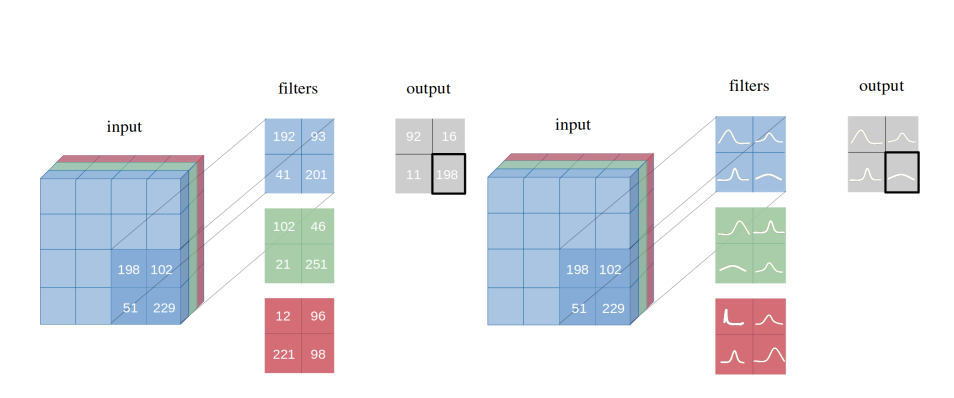
\includegraphics[scale=0.2]{project_img1.png}
        \caption{Input image with exemplary filters and outputs for point-estimates (left) and probability distributions (right) over weights}
        \label{fig1}
    \end{figure}
    \begin{itemize}
        \item In Bayesian approach we try to approximate the intractable true probability distribution $p(w|D)$ with the variational probability distributions $q_\theta(w|D)$
    \end{itemize}
\end{frame}
\begin{frame}{Bayes by backprop - Introduction}
    \begin{itemize}
        \item Bayes by backprop is a variational inference method to learn the posterior distribution on the weights $w \sim q_\theta (w|D)$ of a NN from which $w$ can be sampled during backpropagation.
        \item We try to minimize the KL divergence between the intractable true posterior $p(w|D)$ and the approximate distribution $q_\theta(w|D)$.
        \item The optimal parameters $\theta^{opt}$ can be defined as
        \begin{align*}
            \theta^{opt} &= \argmin_\theta KL [q_\theta(w|D) || p(w|D)]\\
            &= \argmin_\theta KL [q_\theta(w|D) || p(w)] - \mathbb{E}_{q_\theta(w|D)} [log p(w|D)]+log\:p(D) \numberthis{\label{eq1}}\\ 
        \end{align*}
        \item the KL divergence is defined as 
        \begin{align*}
            KL[q_\theta(w|D)||p(w)] = \int q_\theta(w|D) log \frac{q_\theta(w|D)}{p(w)} d\theta \numberthis{\label{eq2}}
        \end{align*}
    \end{itemize}
\end{frame}
\begin{frame}{Variational free energy}
    \begin{itemize}
        \item The cost function $ KL [q_\theta(w|D) || p(w)] - \mathbb{E}_{q_\theta(w|D)} [log p(w|D)]+logp(D)$ is widely known as \emph{variational free energy}.
        \item The first term $ KL [q_\theta(w|D) || p(w)]$ is dependent on the definition of prior $p(w)$ and thus called complexity cost and the next term $\mathbb{E}_{q_\theta(w|D)} [log p(w|D)]$ is dependent on the data $p(D|w)$, thus called the likelihood cost. The term $log p(D)$ is a constant and can be omitted in optimization.
        \item The KL divergence also is intractable to compute exactly. We follow a stochastic variational method and consequently reach at a tractable cost that can be optimized with respect to $\theta$ during training.
        \begin{align*}
            F(D,\theta) \approx \Sigma_{i=1}^{n} log q_\theta (w^{(i)}|D) - log p(w^{(i)}) - log p(D|w^{(i)}) \numberthis{\label{eq3}} \\
        \end{align*}
        where n is the no. of draws. We sample $w(i)$ from $q_\theta(w|D)$.
    \end{itemize}
\end{frame}
\begin{frame}{Local reparameterization trick}
    \begin{itemize}
        \item During implementation, we utilize the local reparameterization trick. We do not sample $w$, but we sample layer activations b instead due to its consequent computational accleration.
        \item The variational posterior probability distribution $q_\theta(w_{ijhw}|D)=\mathcal{N}(\mu_{ijhw},\alpha_{ijhw}\mu^2_{ijhw})$ (where i is the input layer, j is the output layer, h and w are the height and width of the filter respectively) allows to implement the local reparametrization trick in convolutional layers.
        \item The above results leads to the following equation 
        \begin{align*}
            b_j = A_i \circledast \mu_i + \epsilon \odot \sqrt{A_i^2 \circledast (\alpha_i \odot \mu_i^2)} \numberthis{\label{eq4}} 
        \end{align*}
        where $\circledast$ is convolution and $\odot$ is component-wise multiplication.
    \end{itemize}
\end{frame}
\begin{frame}{Uncertainty estimation in Bayesian CNN's}
    In classification tasks we are interested in the predictive distribution $p_D(y^*|x^*)$, where $x^*$ is an unseen data example and $y^*$ is its predicted class. For a Bayesian neural network, this quantity is given by - \begin{align*}
        p_D(y^*|x^*) = \int p_w (y^*|x^*) p_D(w) dw \numberthis{\label{eq5}}
    \end{align*}
    In Bayes by Backprop, Gaussian distribution $q_\theta(w|D)\sim \mathcal{N}(w|\mu,\sigma^2)$, where $\theta={\mu,\sigma}$ are learned with some dataset $D=\{x_i,y_i\}_{i=1}^{n}$. Due to discrete finite nature of most classification tasks, the predictive distribution is commonly assumed to be categorical. Incorporating this we get 
    \begin{align*}
        p_D(y^*|x^*) &= \int Cat(y^*|f_w(x^*))\mathcal{N}(w|\mu,\sigma^2) dw\\
        &=\int \prod_{c=1}^C f(x_c^*|w)^{y_c^*} \frac{1}{\sqrt{2\pi\sigma^2}}e^{\frac{(w-\mu)^2}{2\sigma^2}} \numberthis{\label{eq6}}
    \end{align*}
\end{frame}
\begin{frame}{Continued}
    where $C$ is the total no. of classes and $\Sigma_c f(x_c^*|w)=1$.
    There is no closed form solution due to lack of conjugacy between Categorical and Gaussian distribution. However we can construct an unbiased estimator of the expectation by sampling from $q_\theta(w|D)$.
    \begin{align*}
        \mathbb{E}_q[p_D(y^*|x^*)] = \int q_\theta (w|D) p_w(y|x) dw \approx \frac{1}{T} \Sigma_{t=1}^T\: p_{w_t}(y^*|x^*) \numberthis{\label{eq7}}
    \end{align*}
    where T is the predefined no. of samples.
\end{frame}
\begin{frame}{Continued}
    The variance of the estimator allows us to calculate the uncertainty of our predictions, hence called \emph{predictive variance} and is denoted as -
    \begin{align*}
        Var_q(p(y^*|x^*)) &= \mathbb{E}_q[y^* y^{*T}] - \mathbb{E}_q[y^*]\mathbb{E}_q[y^*]^T \\
        &= \int [diag(\mathbb{E}_p[y^*])-\mathbb{E}_p[y^*]\mathbb{E}_p[y^*]^T] q_\theta (w|D) dw \\
        &+ \int (\mathbb{E}_p[y^*]-\mathbb{E}_q[y^*]) (\mathbb{E}_p[y^*]-\mathbb{E}_q[y^*])^T q_\theta(w|D) \numberthis{\label{eq8}}dw
    \end{align*}
    where $\mathbb{E}_p[y*]=\mathbb{E}_{p(y^*|x^*)}[y^*]$ and $\mathbb{E}_q[y^*]=\mathbb{E}_{q_\theta (y^*|x^*)}[y^*]$
\end{frame}
\begin{frame}{Continued}
    \begin{itemize}
        \item The first term on the right hand side is aleatoric uncertainty (a measure for the variation of "noisy" data) and epistemic uncertainty (caused by the model). By comparing these two values one can see whether the quality of the data is low (high aleatoric uncertainity) or the model itself is the cause for poor performances (high epistemic uncertainty).
        \item The former can be improved by gathering more data whereas the latter requires that the model is refined.
    \end{itemize}
\end{frame}
\begin{frame}{Estimator for variance}
The following estimator is used for the variance - 

\begin{align*}
    Var_q (p(y^*|x^*))  = \frac{1}{T} \Sigma_{t=1}^T diag(\hat{\sigma}_t^2) + \frac{1}{T} \Sigma_{t=1}^T (\hat{\mu}_t-\bar{\mu}) (\hat{\mu}_t-\bar{\mu})^T \numberthis{\label{eq9}}
\end{align*}
where $\hat{\mu}_t$ and $\hat{\sigma}_t^2$ are the mean and variance of the logits and $\bar{\mu} = \hat{\mu}_t/T$.
A better estimator is the following - 
    \begin{align*}
    Var_q (p(y^*|x^*))  = \frac{1}{T} \Sigma_{t=1}^T diag(\hat{p}_t)-\hat{p_t}\hat{p_t}^T + \frac{1}{T} \Sigma_{t=1}^T (\hat{p}_t-\bar{p}) (\hat{p}_t-\bar{p})^T \numberthis{\label{eq10}}
\end{align*}
where $\bar{p} = \hat{p}_t/T$ and $\hat{p}=Softmax(f_{w_t}(x^*))$.
\end{frame}
\begin{frame}{Softplus}
    \begin{itemize}
        \item In this paper the authors defined the doftplus function as below -
        \begin{align*}
            Softplus(x) = \frac{1}{\beta}.log(1+exp(\beta.x))
        \end{align*}
        default value of $\beta$ is 1.
        \item Deploying the traditional Softmax function at the output layer assumes that the classification is done according to logistic sigmoid function. Applying Softplus removes this additional non-linear transformation. We change $\hat{p}=Softmax(f_{w_t}(x^*))$ to $\hat{p}=Softplus(f_{w_t}(x^*))$ in \eqref{eq10}
        \item The implementation is done in two steps. Softplus function is applied to output layer just as any other layer. Then, the outputs are normalized as below
        \begin{align*}
            y_{norm}^* = \frac{y_c^*}{\Sigma_C y_c^*}
        \end{align*}
    \end{itemize}
\end{frame}
\begin{frame}{Intuition behind Softplus}
\begin{itemize}
    \item We classify according to a categorical distribution, this can be seen as an approximation of the outputs with one-hot vectors. If those vectors already contains a lot of zeros in it, the approximation is going to be more accurate. For a Softmax, predicting zeros requires a logit of $-\infty$, which is hard to achieve in practice. For the Softplus normalization we need a negative value around -4 to get a nearly 0 output. Consequenty, Softplus normalization can easily produce vectors that are in prectice zero, whereas Softmax cannot.
\end{itemize}
\end{frame}
\begin{frame}{Results}
    \begin{figure}
        \centering
        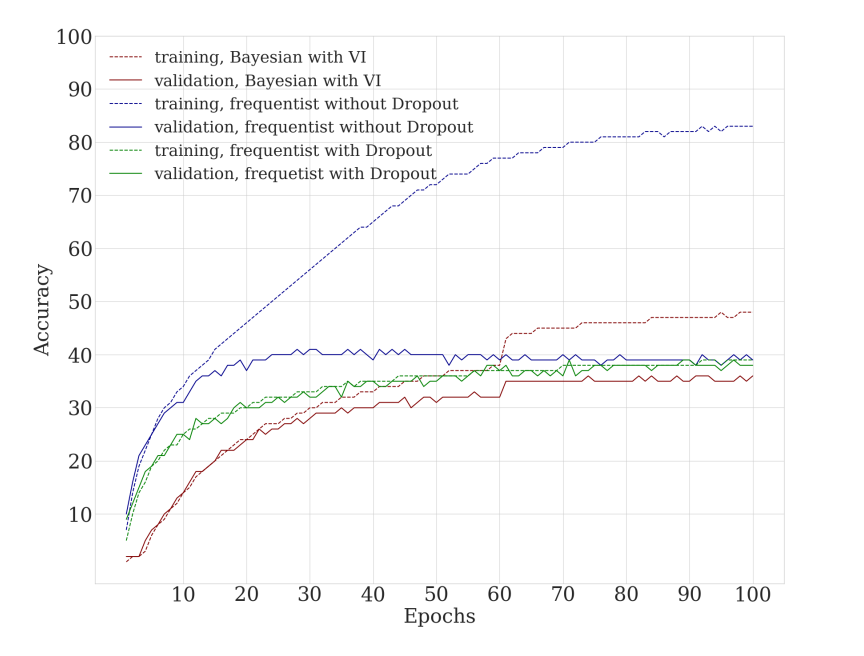
\includegraphics[scale=0.3]{Project_img2.png}
        \caption{AlexNet trained on CIFAR-100 by Bayesian and frequintis inference}
        \label{fig2}
    \end{figure}
\end{frame}
\begin{frame}{Results}
    \begin{figure}
        \centering
        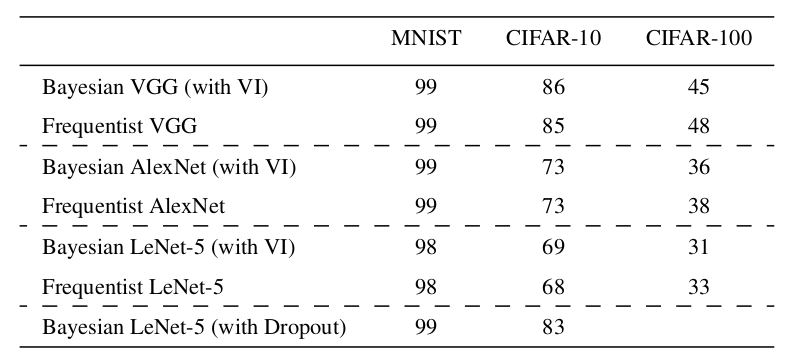
\includegraphics[scale=0.3]{Project_img3.png}
        \caption{Comparison of validation accuracies for different architectures with variational inference and frequentist inference}
        \label{fig3}
    \end{figure}
\end{frame}
\begin{frame}{Results}
    \begin{figure}
        \centering
        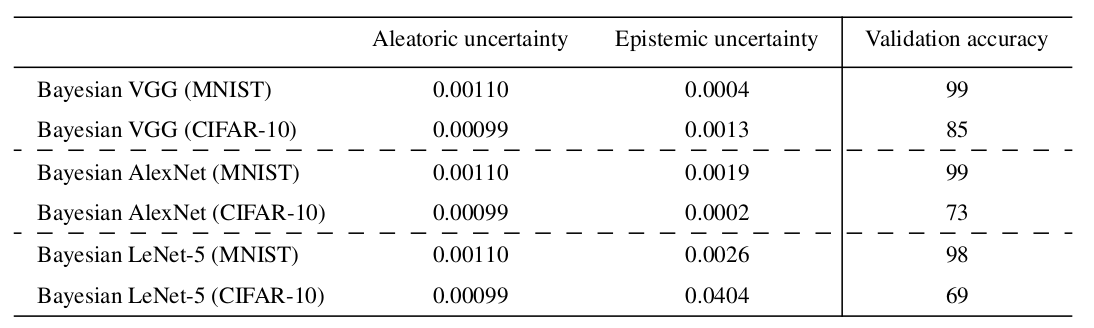
\includegraphics[scale=0.3]{Project_img4.png}
        \caption{Aleatoric and epistemic uncertainity for Bayesian VGG, ALexNet, LeNet-5 calculated for MNIST and CIFAR-10, computed using Softplus normalization}
        \label{fig4}
    \end{figure}
\end{frame}
\begin{frame}{Concluding remarks}
    \begin{itemize}
        \item Bayesian CNNs trained by variational inference achieve valiadation accuracies comparable to the ones trained by frequentist inference. 
        \item Bayesian networks incorporate naturally effects of regularization and are less prone to overfitting compared to frequentists networks.
        \item We see correlating pattern between validation accuracies and epistemic uncertainties, with increasing validation accuracy , epistemic uncertainity decreases.
    \end{itemize}
\end{frame}
\begin{frame}{Appendix}
    Proof of \eqref{eq1}
    \begin{align*}
            KL [q_\theta(w|D) || p(w|D)] &= \int q_\theta(w|D) log \frac{q_\theta(w|D)}{p(w|D)} d\theta \\
            &= \int q_\theta(w|D) log \frac{q_\theta(w|D) p(D)}{p(D|w)p(w)} d\theta\\
            &= \int q_\theta(w|D) log \frac{q_\theta(w|D)}{p(w)} d\theta + \mathbb{E}_q[log \:p(D)]\\
            &- \mathbb{E}_q[log p(D|w)]\\
            &= KL [q_\theta(w|D) || p(w)] - \mathbb{E}_{q_\theta(w|D)} [log p(w|D)]\\
            &+log\:p(D)
    \end{align*}
\end{frame}
\begin{frame}{References}
    \begin{itemize}
        \item \href{https://arxiv.org/pdf/1806.05978v6.pdf}{Uncertainity Estimations by Softplus normalization in Bayesian Convolutional Neural Networks with Variational Inference Kumar Shridhar, Felix Laumann}
    \end{itemize}
\end{frame}
\end{document}